\documentclass[12pt]{jreport}

\usepackage{paper}
\usepackage{afterpage}
\usepackage{pxjahyper}
\hypersetup{
	colorlinks=false, % リンクに色をつけない設定
	bookmarks=true, % 以下ブックマークに関する設定
	bookmarksnumbered=true,
	pdfborder={0 0 0},
	bookmarkstype=toc
}

\begin{document}

%%●●●●●●●●●●●●●●●●●●●●●●●●●●●●●●●●●●●
%% 目次
%% ページ番号をローマ数字にする.

\newpage
\setcounter{page}{0}
\pagenumbering{roman}
\tableofcontents

%%●●●●●●●●●●●●●●●●●●●●●●●●●●●●●●●●●●●
%% ページ番号をアラビア数字に戻す.
\newpage
\setcounter{page}{1}
\pagenumbering{arabic}


%%●●●●●●●●●●●●●●●
\chapter{2週目 ツールを用いた回路設計技術}
\section{目的}
  1週目では紙の上で回路設計を行ったが,巨大なシステム,例えばGPU\footnote{Graphics Processing Unitの略} などを
    紙上で設計することは困難であり,コンピュータを用いて設計することが一般的である.
  2週目では,近年の回路設計技術に対する理解を深めるために,Windowsツール,Xilinx ISE WebPACKを用いて回路設計を行う.
  また,回路シミュレータ上で動作検証を行う.

  \subsection{Xilinx ISE WebPACKについて}
  一般に集積回路の制作には時間がかかり,また大量生産を行わない限りコストもかかるため,
  少量生産を行う際はFPGA\footnote{Field Programmable Gate Arrayの略} など論理回路をエミュレートできる回路が使用される.
  Xilinx は FPGA の大手メーカであり,ISE WebPACK は Xilinx が提供する.

\section{実験方法}
シミュレーションで使用するデバイスは Spartan3E ファミリの XC3S100E の CP132 パッケージである.
Xilinxの回路図ベースで実験を進めていく.
\subsection{課題1 3入力多数決回路}
3入力多数決回路の回路を作成する.真理値表を表\ref{tab:TMR}に示す.
\begin{table}[htb]
  \centering
  \caption{多数決回路の真理値表}
  \label{tab:TMR}
  \begin{tabular}{ccc|c}
    $A$ & $B$ & $C$ & $Y$ \\ \hline
     0  &  0  &  0  &  0  \\
     0  &  0  &  1  &  0  \\
     0  &  1  &  0  &  0  \\
     0  &  1  &  1  &  1  \\
     1  &  0  &  0  &  0  \\
     1  &  0  &  1  &  1  \\
     1  &  1  &  0  &  1  \\
     1  &  1  &  1  &  1  \\
  \end{tabular}
\end{table}
設計した回路図を\ref{fig:TMRsch}に示す.
シミュレーションのテストベンチを付録のソースコード\ref{lst:tmrtestbench}に示す.

\begin{figure}[tbp]
   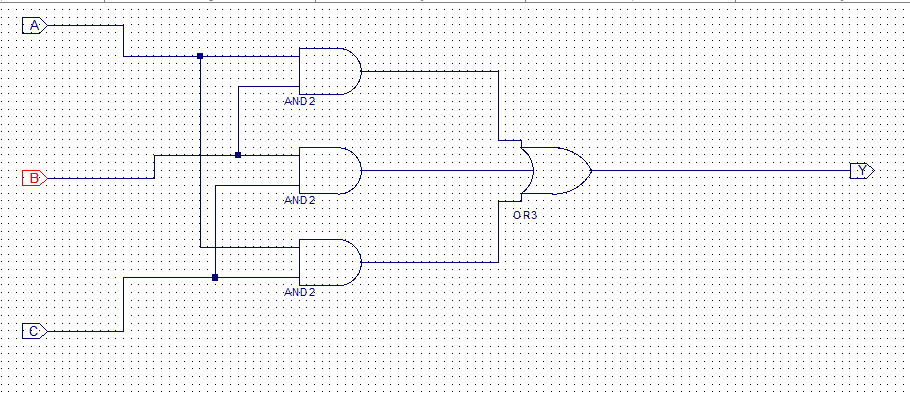
\includegraphics[width=150mm,angle=0]{week2/pics/TMRsch.png}
   \caption{3入力多数決回路の回路図} %タイトルをつける
   \label{fig:TMRsch} %ラベルをつけ図の参照を可能にする
\end{figure}

\subsection{課題2 発展課題 10進7セグデコーダの制作}
7セグメントデコーダを作成する.$I_0$から$I_3$の入力で7セグメント LED のセグメントの出力を得るようにする.
設計する回路は,正論理を仮定すると,アノードコモンの7セグメント LED は0のときに光るようにする.
そのため真理値表は表\ref{tab:7segdec}のとおりである.
カルノー図を半自動生成するために Excel を用いて表を生成している(図\ref{fig:7seg-dec-des}).
シミュレーションのテストベンチを付録のソースコード\ref{lst:schbased7segtestbench}に示す.

\begin{table}[htb]
  \centering
  \caption{7セグデコーダの真理値表}
  \label{tab:7segdec}
  \begin{tabular}{c||cccc||ccccccc}
     N &$I_3$&$I_2$&$I_1$&$I_0$&$A$&$B$&$C$&$D$&$E$&$F$&$G$ \\ \hline
     0 & 0  &  0  &  0  &  0 & 0 & 0 & 0 & 0 & 0 & 0 & 1 \\
     1 & 0  &  0  &  0  &  1 & 1 & 0 & 0 & 1 & 1 & 1 & 1 \\
     2 & 0  &  0  &  1  &  0 & 0 & 0 & 1 & 0 & 0 & 1 & 0 \\
     3 & 0  &  0  &  1  &  1 & 0 & 0 & 0 & 0 & 0 & 0 & 1 \\
     4 & 0  &  1  &  0  &  0 & 1 & 0 & 0 & 1 & 1 & 0 & 0 \\
     5 & 0  &  1  &  0  &  1 & 0 & 1 & 0 & 0 & 1 & 0 & 0 \\
     6 & 0  &  1  &  1  &  0 & 0 & 1 & 0 & 0 & 0 & 0 & 0 \\
     7 & 0  &  1  &  1  &  1 & 0 & 0 & 0 & 1 & 1 & 1 & 1 \\
     8 & 1  &  0  &  0  &  0 & 0 & 0 & 0 & 0 & 0 & 0 & 0 \\
     9 & 1  &  0  &  0  &  1 & 0 & 0 & 0 & 0 & 1 & 0 & 0 \\
  \end{tabular}
\end{table}

\begin{figure}[tbp]
   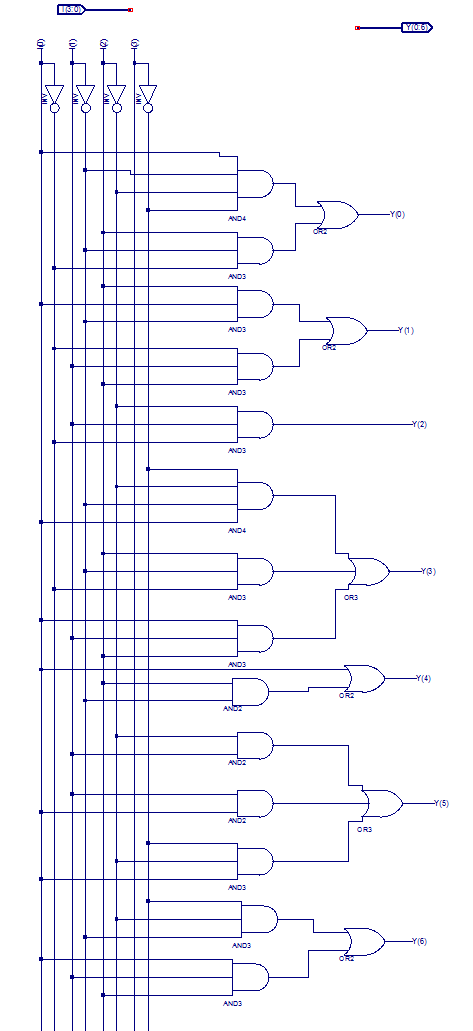
\includegraphics[height=230mm,angle=0]{week2/pics/7seg-sch.png}
   \caption{7セグデコーダの回路図} %タイトルをつける
   \label{fig:7seg-dec-sch} %ラベルをつけ図の参照を可能にする
\end{figure}

\begin{figure}[tbp]
   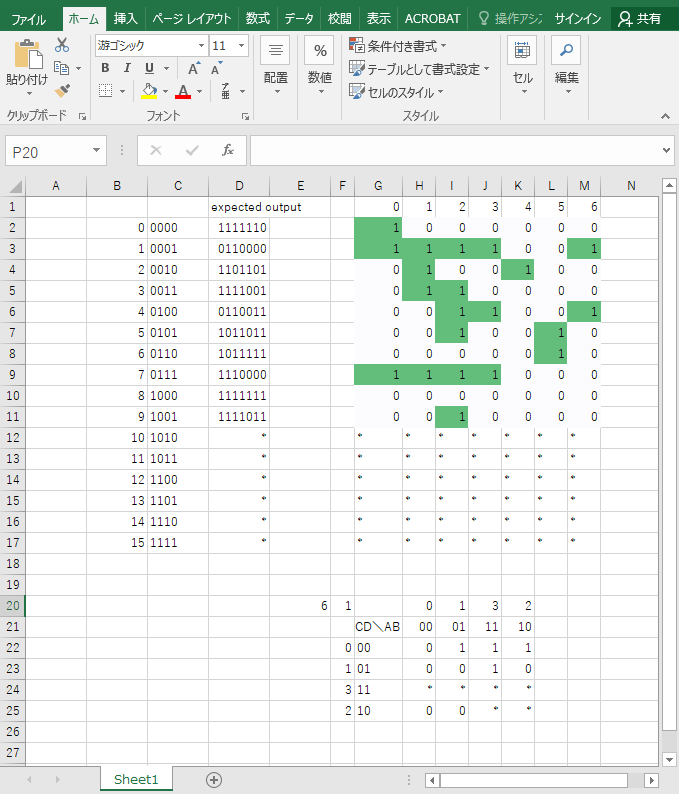
\includegraphics[width=150mm,angle=0]{week2/pics/designingprocess.png}
   \caption{7セグデコーダの設計に用いたシート, 画像では6のカルノー図が出力されている} %タイトルをつける
   \label{fig:7seg-dec-des} %ラベルをつけ図の参照を可能にする
\end{figure}


\subsection{課題3 2入力ANDゲートのFPGAボードでの動作確認}
2入力ANDゲートを実際に作成し,その入力を押しボタンスイッチ,出力をLEDに接続し,入出力を割り当て,
コンフィグレーションデータを作成する.
作成したデータをFPGAにダウンロードし,動作検証をする.
回路図を図\ref{fig:ANDsch}に示す.ピンのa割り当てを図\ref{fig:ANDpinasign}に示す.

\begin{figure}[tbp]
  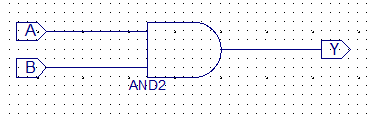
\includegraphics[width=100mm,angle=0]{week2/pics/ledswandsch.png}
  \centering
   \caption{ANDゲートの回路図} %タイトルをつける
   \label{fig:ANDsch} %ラベルをつけ図の参照を可能にする
\end{figure}


\begin{figure}[tbp]
  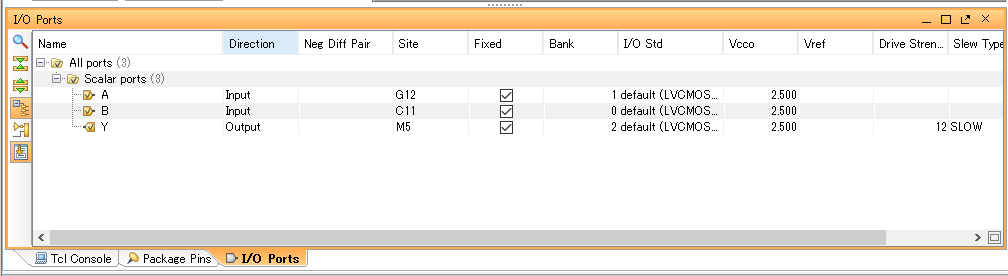
\includegraphics[width=140mm,angle=0]{week2/pics/pinasign.png}
  \centering
   \caption{ANDゲートのピンアサイン} %タイトルをつける
   \label{fig:ANDpinasign} %ラベルをつけ図の参照を可能にする
\end{figure}

\clearpage
%==============================================
\section{実験結果}

\subsection{課題1 3入力多数決回路}
シュミュレーション結果を図\ref{fig:tmrsim}に示す.

\begin{figure}[tbp]
  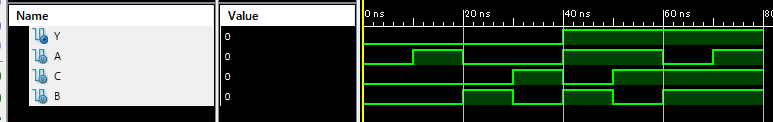
\includegraphics[width=140mm,angle=0]{week2/pics/TMRsim.png}
  \centering
   \caption{3入力多数決回路のシュミュレーション結果} %タイトルをつける
   \label{fig:tmrsim} %ラベルをつけ図の参照を可能にする
\end{figure}


\subsection{課題2 発展課題 10進7セグデコーダの制作}
シュミュレーション結果を図\ref{fig:schbased7segsim}に示す.
テストベンチの結果の中で,赤で引かれた線に注目すると,7セグのデコード結果が見える.
\begin{figure}[tbp]
  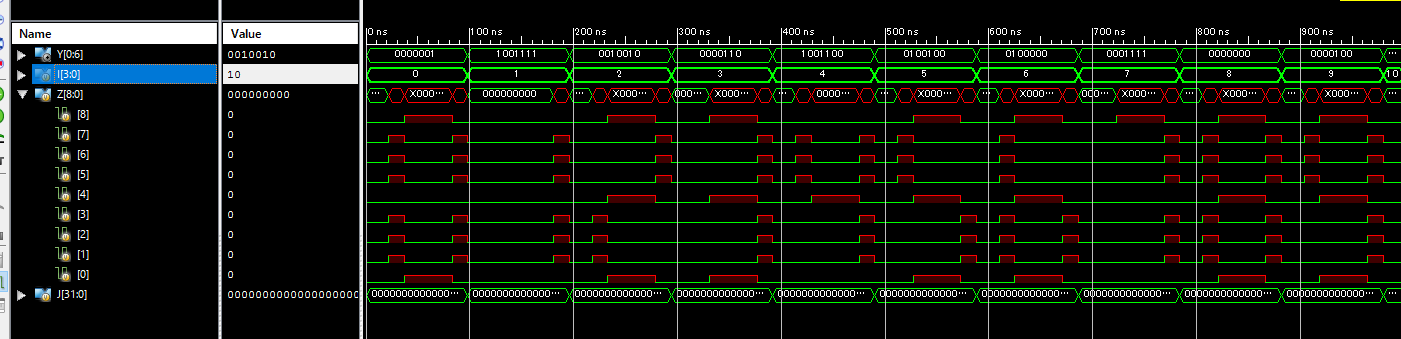
\includegraphics[width=140mm,angle=0]{week2/pics/waveform-7seg.png}
  \centering
   \caption{7セグメントデコーダのモジュールテスト} %タイトルをつける
   \label{fig:schbased7segsim} %ラベルをつけ図の参照を可能にする
\end{figure}


\subsection{課題3 2入力ANDゲートのFPGAボードでの動作確認}
動作確認をしている様子を図\ref{fig:LEDANDex}に示す.
2つのボタンを0個または1個押したときにはLEDは点灯せず,両方のボタンを押したときのみLEDが点灯した.

\begin{figure}[tbp]
  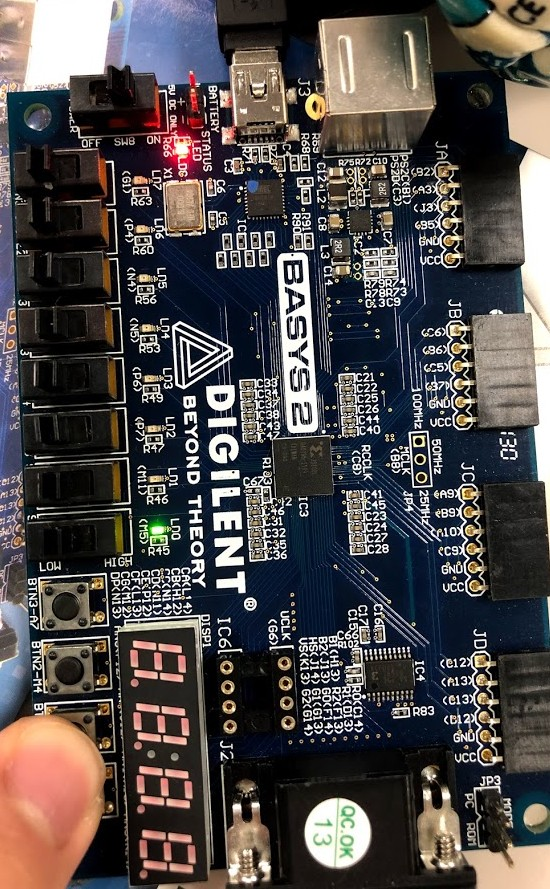
\includegraphics[angle=90,width=140mm]{week2/pics/LEDAND.jpg}
  \centering
   \caption{2入力ANDのLEDへの出力テスト} %タイトルをつける
   \label{fig:LEDANDex} %ラベルをつけ図の参照を可能にする
\end{figure}

\section{考察}
\subsection{課題1 3入力多数決回路}
3入力多数決回路について,予想通りの動作ができていることがわかる.
この回路で,信頼性が求められる計算の正確性が確保できると考えられる.

\subsection{課題2 発展課題 10進7セグデコーダの制作}
7セグメントデコーダも,波形から正しくデコードできている様子がわかる.
0 で光るように設計したため,ANDベースで設計する際に論理素子が少なくて済んだ.
これも,光る部分の設計より,光らない部分を考えたほうが回路が簡略化しやすいことが理由としてある.

\subsection{課題3 2入力ANDゲートのFPGAボードでの動作確認}
2入力 AND 回路について,想定通り両方のボタンを押したときのみLEDが光った.
これは,スイッチが押されたら1,LEDも1のときに光るように設計されているためである.

\section{感想}
コンピュータ上での回路設計に触れることができ,基本的なFPGAの特性をつかむことができた.
特に実際に回路をブレッドボードと論理ゲートで組むことなく,複雑な回路のエミュレートが実機レベルで開発できる点から,
FPGAは有用だと思う.

7セグメントデコーダの制作では,どのセグを光らせるのか,迷う部分があった.
例えば1, 6, 7, 9などは光らせ方が複数あり\footnote{数字''1''は右左の違い,6, 7, 9 はそれぞれA,F,Dセグメントの発光の有無に迷う},
それぞれの数字において,発光パターンが複数考えられたが,
解説に揃えて設計することにした.後の検算のことを考えてのことである.

あと,レポート作成時にTexで表作るのが意外と大変だった.
Excel等で作った表を変換するソフトを用意すべきだと思った.

\clearpage
\section{付録}
\lstinputlisting[caption=TMRのテストベンチ,label=lst:tmrtestbench]{week2/program/TMRtestbench.v}
\lstinputlisting[caption=回路図で設計した7セグデコーダのテストベンチ,label=lst:schbased7segtestbench]{week2/program/schbased7segtestbench.v}
  

\chapter{3週目 Verilog を用いた回路設計技術}
\section{目的}
2週目の実験では,コンピュータ上で回路図を設計した.しかし大規模な回路の制作に回路図は向いていない.
多くの場合,ハードウェア記述言語 (HDL; Hardware Description Language) を用いて記述される.
3週目は HDL の1種である Verilog を用いて回路設計を行う.
Verilog は C言語と似た言語であり,C言語習得者にとっては感覚的に扱いやすい言語である.

\section{実験方法}

\subsection{課題1 全加算器}
半加算器,全加算器を Verilog で記述する.ただし手続きブロックと算術演算子を用いてはならない.
ここで全加算器は,A, B, $C_I$の入力の和を求める回路である.
全加算器の真理値表を\ref{tab:FA}に示す.

\begin{table}[htb]
  \centering
  \caption{全加算器の真理値表}
  \label{tab:FA}
  \begin{tabular}{ccc|cc}
    $A$ & $B$ & $C_I$ & $C_O$ & $S$ \\ \hline
     0  &  0  &  0  &  0    &  0\\
     0  &  0  &  1  &  0    &  1\\
     0  &  1  &  0  &  0    &  1\\
     0  &  1  &  1  &  1    &  0\\
     1  &  0  &  0  &  0    &  1\\
     1  &  0  &  1  &  1    &  0\\
     1  &  1  &  0  &  1    &  0\\
     1  &  1  &  1  &  1    &  1\\
  \end{tabular}
\end{table}

ソースコードをソースコード\ref{lst:FA-source}に示す.
テストベンチをソースコード\ref{lst:FA-testbench}に示す.


\subsection{課題2について}
課題2は選択問題だが,実験時間が余ったため,両方とも実験を行った.両方ともレポートにまとめておく.

\subsection{課題2A 4ビット加減算器}
4ビット加減算器を作成する.加減算機とは,制御入力の値に応じ,加算器または減算器となる回路である.
減算は,$S=A-B$などという式に対し,2の補数表現を用いて$C = -B = (B \oplus 4'hF) + 1$と変形することで,
$S=A+C$という式で記述することができる.
%
そのため,通常の加算器に対し,XORを通して符号を反転させ,
全加算器の0ビット目のキャリービットを1にすることで,減算器を実現することができる.
図\ref{fig:fa-sign-sch}に回路図を示す.図中,FAは全加算器という意味である.
\begin{figure}[tbp]
  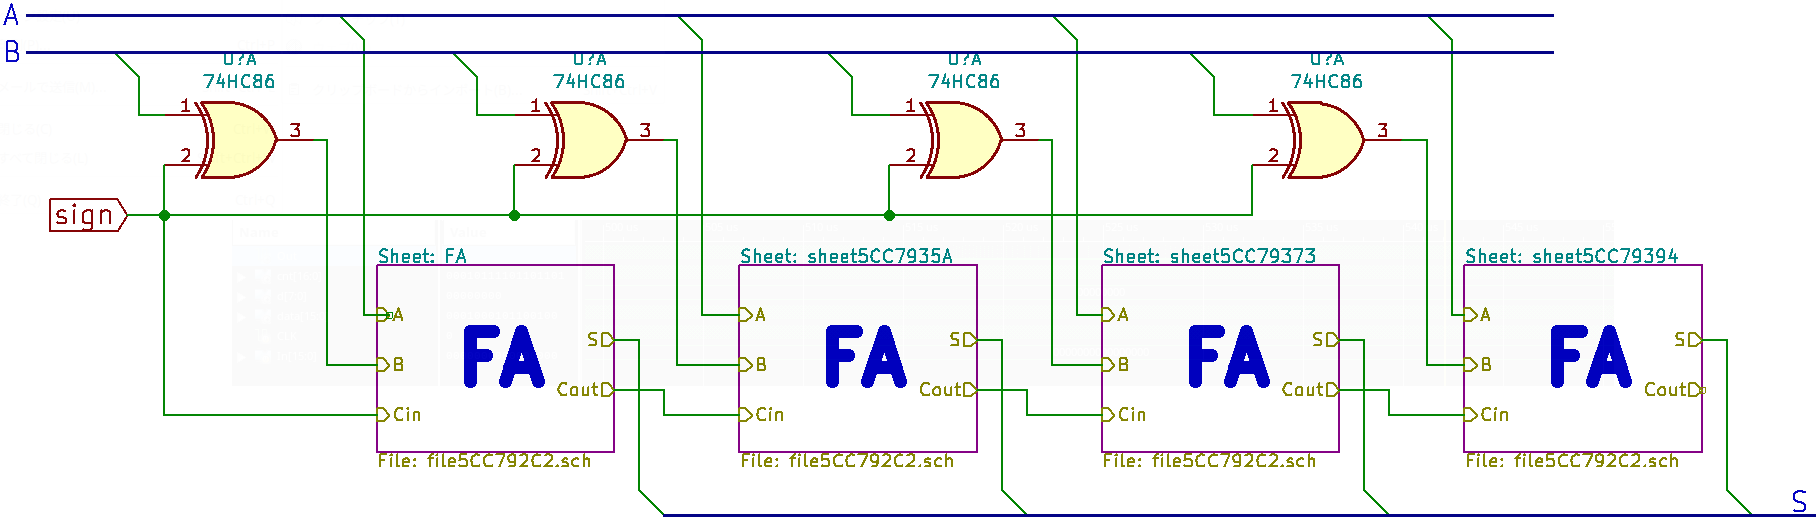
\includegraphics[angle=0,width=160mm]{week3/pics/FA-sign-sch.png}
  \centering
   \caption{加減算器の構成} %タイトルをつける
   \label{fig:fa-sign-sch} %ラベルをつけ図の参照を可能にする
\end{figure}
実際には,最終ビットのキャリービットの出力もモジュールから出力させる.

ソースコードをソースコード\ref{lst:addsub-source}に示す.
テストベンチをソースコード\ref{lst:addsub-testbench}に示す.


\subsection{課題2B 4ビット乗算器}
符号なし4ビット乗算器を制作する.4ビットの掛け算の積は8ビットとなる.
2進数での掛け算は,10進法での筆算と同じように行う(表\ref{tab:binarymult}).

\begin{table}[htb]
  \centering
  \caption{2進法での筆算例}
  \label{tab:binarymult}
  \begin{tabular}{ccccccccc}
     & & & &1&0&1&0&\\
     & & &$\times$&0&1&0&1&\\ \hline
     & & & &1&0&1&0&(1)\\
     & & &0&0&0&0& &(0)\\
     & &1&0&1&0& & &(1)\\
    +&0&0&0&0& & & &(0)\\ \hline
     &0&1&1&0&0&1&0&\\
  \end{tabular}
\end{table}

具体的には,$C=A\times B$の演算に対して,$A$を左にシフトしつつ,$B$の各ビットで全体をマスクし,最後に合算する.
筆算例とHDLで記述されたソースコードを合わせて見ながら理解してもらいたい.
ソースコードをソースコード\ref{lst:handmult-source}に示す.
テストベンチをソースコード\ref{lst:handmult-testbench}に示す.


\subsection{課題3 手続きブロックを用いた7セグメントデコーダの作成}
2週目の課題にあった7セグメントLED用のデコーダを手続きブロックを用いて記述する.
ソースコードをソースコード\ref{lst:block-7segled-source}に示す.
テストベンチをソースコード\ref{lst:block-7segled-testbench}に示す.


\subsection{課題4 7セグメントLEDへの出力と発光の関係の観察}
7セグメントLEDの光り方を調べるため,7セグメントLEDとスイッチをバッファで連結し,光り方を観察する.

ピンの割り当ては,詳細は付録にまとめておく(ソースコード\ref{lst:check-7segled-pinasign}).
ボタンとLEDへの出力の光らせ方も,ソースコード\ref{lst:check-7segled-source}で記述している.

7セグメントLEDはアノードコモンである.
カソード側はAセグメントからG,dotのLEDに繋がっていて,4桁すべて同じ端子を共有している.
プッシュスイッチ側スイッチはプルダウン抵抗を通して何も押されない状態では0出力となる.
IOの割り当てでは,スライドスイッチをLEDのカソード側8ビットに割り当てをした.
プッシュスイッチは,アノード側に4桁分配置した.

7セグメントLEDの光り方を調べる前に期待される動作を考える.
7セグメントLEDのアノード側は Low 状態で光る状態の準備ができる.
カソード側はHigh状態になることで光る準備ができ,
両方が成立したセグメントのLEDが発光することが期待できる.

そのため,まずはプッシュボタンは何も押さず,すべての桁を選択した状態でテストを開始する.
スライドスイッチとLEDの発光の関係を調査する.
その次にスライドスイッチはすべてHighの状態にし,スライドスイッチを1つずつ押して,桁が無効になるかを観察する.

\subsection{課題5 7セグメントLED表示回路の作成}
7セグメントLEDへ実際の数値のの出力をテストする.
押しボタン3つを3ビットの入力とし,それに応じた数字をすべての桁の7セグメントLEDに出力する回路を作成する.

7セグメントLEDとスイッチのピン割り当てをソースコード\ref{lst:check-7segledx1111-pinasign}に示す.
その他の7セグメントLEDの表示ソースコードを\ref{lst:check-7segledx1111-source}に示す.


\subsection{課題6 乗算における符号について}
4ビット乗算器について,符号ありと符号なし両方の演算結果の違いを観測する.
ソースコードをソースコード\ref{lst:multitest-source}に示す.
テストベンチをソースコード\ref{lst:multitest-testbench}に示す.


%% \clearpage
%==============================================
\section{実験結果}
\subsection{課題1 全加算器}
シミュレーション結果の波形を図\ref{fig:adder-sim}に示す.

\begin{figure}[tbp]
  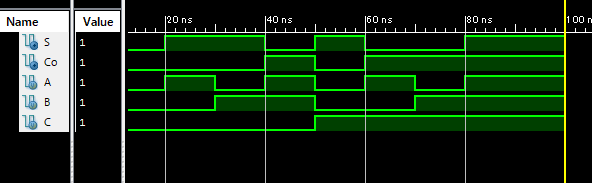
\includegraphics[angle=0,width=140mm]{week3/pics/adder-sim.png}
  \centering
  \caption{全加算器のモジュールテスト} %タイトルをつける
  \label{fig:adder-sim} %ラベルをつけ図の参照を可能にする
\end{figure}


\subsection{課題2A 4ビット加減算器}
Bの符号を正のまま,つまり加算中のシミュレーション結果の1部の波形を図\ref{fig:addersub-add-sim}に示す.
Bの符号を負にし,減算中のシミュレーション結果の1部の波形を図\ref{fig:addersub-sub-sim}に示す.
波形中,SIGNが符号を示しており,すべてのデータは符号ありと仮定して表示している.出力Cは桁溢れを示している.
図中,変数J, K, SIはループ変数で特に意味はない.

\begin{figure}[tbp]
  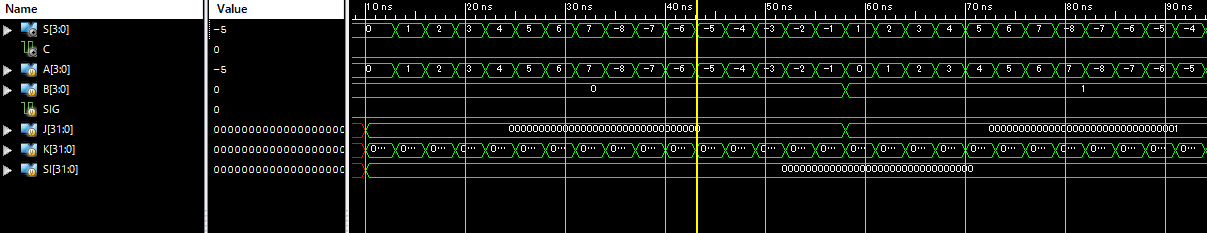
\includegraphics[angle=0,width=160mm]{week3/pics/addersub-add-sim.png}
  \centering
  \caption{加減算器の加算時のモジュールテスト} %タイトルをつける
  \label{fig:addersub-add-sim} %ラベルをつけ図の参照を可能にする
\end{figure}

\begin{figure}[tbp]
  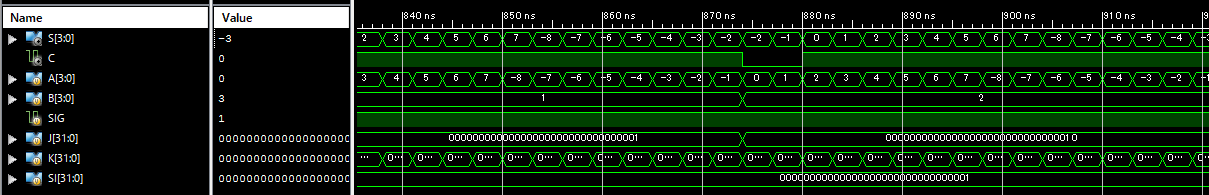
\includegraphics[angle=0,width=160mm]{week3/pics/addersub-sub-sim.png}
  \centering
  \caption{加減算器の減算時のモジュールテスト} %タイトルをつける
  \label{fig:addersub-sub-sim} %ラベルをつけ図の参照を可能にする
\end{figure}


\subsection{課題2B 4ビット乗算器}
4ビット乗算器のモジュールテストの結果の1部を図\ref{fig:handmade-mul-sim}に示す.
図中,変数J, Kはループ変数で特に意味はない.

\begin{figure}[tbp]
  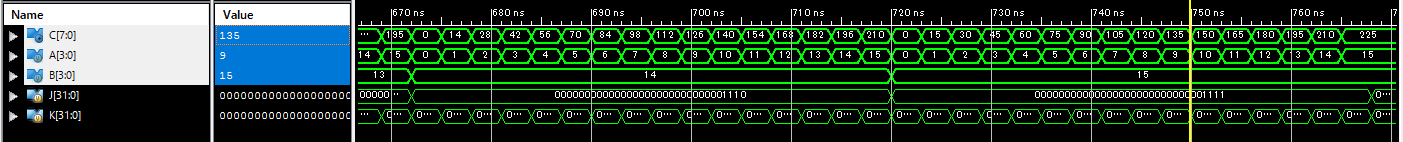
\includegraphics[angle=0,width=160mm]{week3/pics/multi-unsigned-handmade-sim.png}
  \centering
  \caption{4ビット乗算器のモジュールテスト} %タイトルをつける
  \label{fig:handmade-mul-sim} %ラベルをつけ図の参照を可能にする
\end{figure}

\subsection{課題3 手続きブロックを用いた7セグメントデコーダの作成}
7セグデコーダのモジュールテストの結果を図\ref{fig:decode7seg-block}に示す.
2週目の課題同様に赤の線に注目するとデコード結果が見える.
\begin{figure}[tbp]
  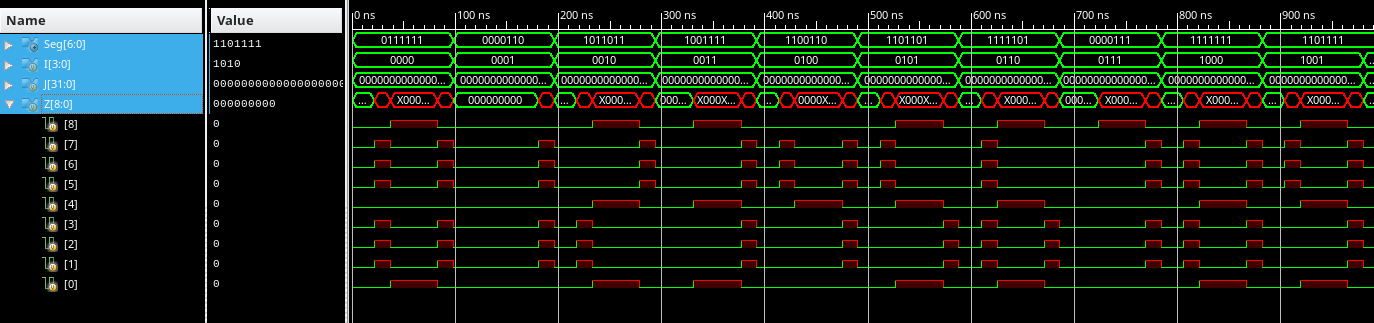
\includegraphics[angle=0,width=160mm]{week3/pics/7seg-dec-sim.png}
  \centering
  \caption{7セグデコーダのモジュールテスト} %タイトルをつける
  \label{fig:decode7seg-block} %ラベルをつけ図の参照を可能にする
\end{figure}

\subsection{課題4 7セグメントLEDへの出力と発光の関係の観察}
出力値と7セグメントLEDの光り方の調査結果を調べた.
実験方法で述べたように,課題4の実験は2つに分けて行われた.

前者のほうでは,プッシュスイッチを押さずにセグメントの発光パターンを調査する.
結果としては,割り当てたセグメントとスライドスイッチの間の関係性が検証できた.
dotに関してはHigh出力のとき,小数点を表現するときに用いられる''.''が現れた.
その他,回路図のセグメントの割り当てと同じようにセグメントがHighで点灯した.

次に後者の方では,スライドスイッチを幾つかHighにセットした状態で1つずつプッシュスイッチを押す.
押すとスイッチの出力はHighになる.
押した桁に対応する桁が消灯した.
4つ全て押すと完全に消灯した.
3つだけ押すと,一つだけ残して消えた.

\subsection{課題5 7セグメントLED表示回路の作成}
7セグメントLEDは目的の動作を果たしていた.0-7のバイナリ入力に対応する7セグメント表示ができていた.

\subsection{課題6 乗算における符号について}
テストベンチの結果を図\ref{fig:mult-sighned-unsigned}に示す.符号を考慮した演算結果になっている.
符号なしでは単に乗算計算をしている.

\section{考察}
\subsection{課題1 全加算器}
1ビットの加算計算ができていることがわかる.

\subsection{課題2A 4ビット加減算器}
4ビットの加減算計算が正しく動作していることがわかる.

\subsection{課題2B 4ビット乗算器}
4ビットの乗算計算が正しく動作していることがわかる.
符号は考慮していないので,符号なしの計算のみしかできない.

\subsection{課題3 手続きブロックを用いた7セグメントデコーダの作成}
7セグメントLED用のデコードが正しく動作していることがわかる.
2週目で設計した回路図と同様の動作をした.
こちらのほうが開発時間がかなり短くなっている.
以前は3時間くらいはかかってたが,今回は20分くらいで同様の動作を実現した.

\subsection{課題4 7セグメントLEDへの出力と発光の関係の観察}
7セグメントLEDの動作として,桁を決めるピンと,7セグメントLEDのセグを制御するポートがあることがわかる.
ポートとセグメントの対応は,回路図通りであることが分かった.
アノード側はLowで光ることがわかる.
カソード側はHighで光る.

両方がANDの条件式になっていて,両方成り立つときのみLEDが点灯する.
セグメントの制御用ポートがすべての桁で共通していることから,
すべての桁を別々に,また同時に制御することはできない.
桁を高速に切り替えながら,それぞれの桁を表示するダイナミック制御を行うことが考えらる.

4桁の7セグメントLEDのように,なにも工夫しないと$(7+1)\times4=32$個のLEDを同時に制御するのには多数のポートが必要になる.
しかしFPGAではポートが有限であるため,1つのLEDに1つのポートを対応させるのは入出力ポートの資源の面から考えると良くない.
この回路で使われているダイナミック点灯の方式では,この場合は$8+4=12$ポートで制御できる.
半分以下までポート数を削減できるが,同時には制御できないので,高速に桁を切り替えながら表示することが考えられる.
そのためデメリットとしてはLEDの輝度が$\frac{1}{4}$まで低下することが考えられる.

\subsection{課題5 7セグメントLED表示回路の作成}
7セグメントLED用の出力を正しく動作している.
今回はcase文で実装しているが,if文でも同様の実装ができることが考えられる.

\subsection{課題6 乗算における符号について}
符号ありと符号なしの乗算の演算結果に違いが出た.
符号ありでは,私たちは普段,符号同士の演算を別にしておいて,後で符号をまとめる.
乗算器でも同様に,符号なしでは符号の計算は考慮されなかった.
すべて符号なしとして処理されている.
逆に符号ありでは,符号を考慮しての計算ができていることがわかる.

\begin{figure}[tbp]
  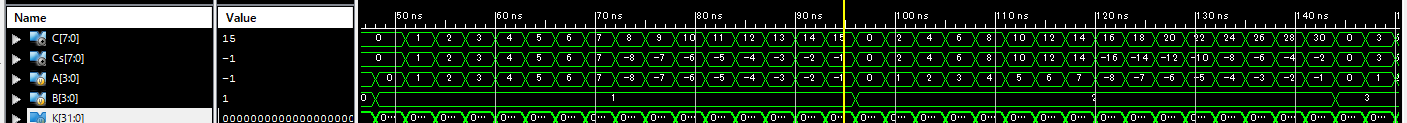
\includegraphics[angle=0,width=160mm]{week3/pics/multi-signed-unsigned.png}
  \centering
  \caption{4ビット乗算器における符号ありと符号なしの違い} %タイトルをつける
  \label{fig:mult-sighned-unsigned} %ラベルをつけ図の参照を可能にする
\end{figure}

\section{感想}
以前7セグメントLED用のデコード回路を作成したときよりもVerilogで記述したほうが製作時間が短くった.
ハードウェアの最適化は人がやるところと機械に任せるところの選定が必要だと思った.
全体の構造は人の手で決めるべきだが,細かい部分はコンピュータの論理合成により行われたほうが簡単にできる.

また,7セグメントLEDの制御回路に工夫が見られた.
ポート数は,マイコンでプログラミングする際にも制約として考慮しなければならないことが多い.
少ないポートで効率よく制御するためには,回路上の工夫が欠かせないことがわかった.

また,加算器に関しては,このままでは桁が長くなると,計算時間が長くなると思った.
桁上がりが入るのが,前の桁を計算しなければ桁上がりがわからないためである.
高速化するには桁上がりを前もって計算するための機構などを用意する必要があると思う.


\clearpage
\section{付録}
\lstinputlisting[caption=課題1 ソースコード,label=lst:FA-source]{week3/source/adder.v}
\lstinputlisting[caption=課題1 テストベンチ,label=lst:FA-testbench]{week3/source/addertestbench.v}

\lstinputlisting[caption=課題2A ソースコード,label=lst:addsub-source]{week3/source/addsub4.v}
\lstinputlisting[caption=課題2A テストベンチ,label=lst:addsub-testbench]{week3/source/addsub4testbench.v}

\lstinputlisting[caption=課題2B ソースコード,label=lst:handmult-source]{week3/source/handmulti.v}
\lstinputlisting[caption=課題2B テストベンチ,label=lst:handmult-testbench]{week3/source/handmulti-testbench.v}

\lstinputlisting[caption=課題3 ソースコード,label=lst:block-7segled-source]{week3/source/seg7decblock.v}
\lstinputlisting[caption=課題3 テストベンチ,label=lst:block-7segled-testbench]{week3/source/7segtestbench.v}

\lstinputlisting[caption=課題4 ピン割り当て,label=lst:check-7segled-pinasign]{week3/source/check7seg.ucf}
\lstinputlisting[caption=課題4 ソースコード,label=lst:check-7segled-source]{week3/source/check7seg.v}

\lstinputlisting[caption=課題5 ピン割り当て,label=lst:check-7segledx1111-pinasign]{week3/source/seg7proc.ucf}
\lstinputlisting[caption=課題5 ソースコード,label=lst:check-7segledx1111-source]{week3/source/seg7proc.v}

\lstinputlisting[caption=課題6 ソースコード,label=lst:multitest-source]{week3/source/multitest.v}
\lstinputlisting[caption=課題6 テストベンチ,label=lst:multitest-testbench]{week3/source/multitesttestbench.v}
  

\chapter{4週目 Verilog を用いた順序回路の設計}
\section{目的}
3週目では組み合わせ回路を設計した.
4週目では順序回路の設計を学ぶ.また複雑な順序回路設計を体験する.

\section{実験方法}
\subsection{課題1 10進数カウンタの作成}
10進カウンタを設計する.

ソースコードを付録のソースコード\ref{lst:10counter-source}示す.
テストベンチを付録のソースコード\ref{lst:10counter-testbench}示す.

\subsection{課題2}
回路図(図\ref{fig:no2-sch})の動作を予測し,実際に動作させ確かめてみる.
動作予測としては,2通り考えられる.
図\ref{fig:io-config}に,考えられる回路構成を示す.
この矢印のどちらに配線が入っているかで結果が変わると考えられる.

パターン1では,LEDの負荷によりHigh出力のディレイがかかり,
仮にLEDにHi出力がされていてもその瞬時にはHiと認識できるレベルまで電圧が上がらず,読み出した際にLowとして読み込まれる現象が考えられる.
そのため,ボタンを離したときにLEDが消灯する回数が多くなることが考えられる.

パターン2では,バッファやラッチが挿入されて,出力負荷に関係なく論理レベルが決定される例で,
ボタンを押している間,LEDがルーレットのように25MHzで点滅し,ボタンを離した瞬間の出力を保持し続けるという予想がある.
そのため,押している時間がランダムで十分に長いときに離した瞬間のLEDの値もランダムとなる.

これは出力段にラッチの挿入がない場合に考えられるが,実際の出力をもとにした論理合成が行われると起こりうる.
多くのマイクロコントローラでも同様の問題が提起されており,PICコントローラの場合は後続のチップではDラッチを搭載することで問題を回避した.

仮にこのような現象が起きた場合,同条件のもとでもHighになる確率とLowになる確率が同じにならない.
\begin{figure}[tbp]
  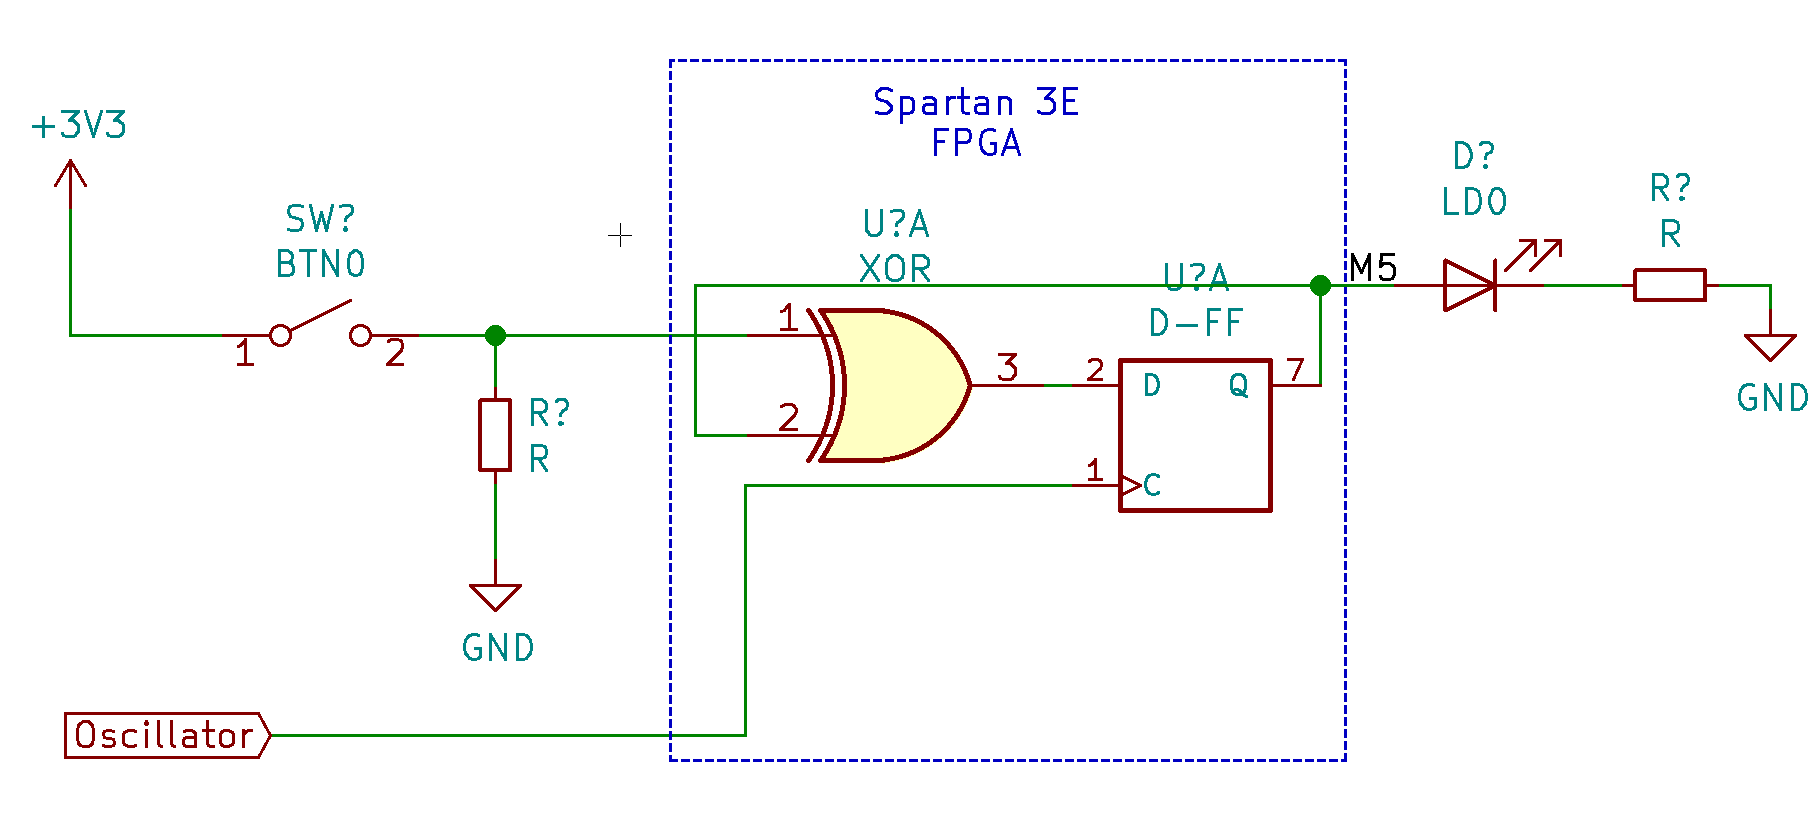
\includegraphics[angle=0,width=160mm]{week4/pics/no2-schematics.png}
  \centering
  \caption{課題2の回路図} %タイトルをつける
  \label{fig:no2-sch} %ラベルをつけ図の参照を可能にする
\end{figure}

\begin{figure}[tbp]
  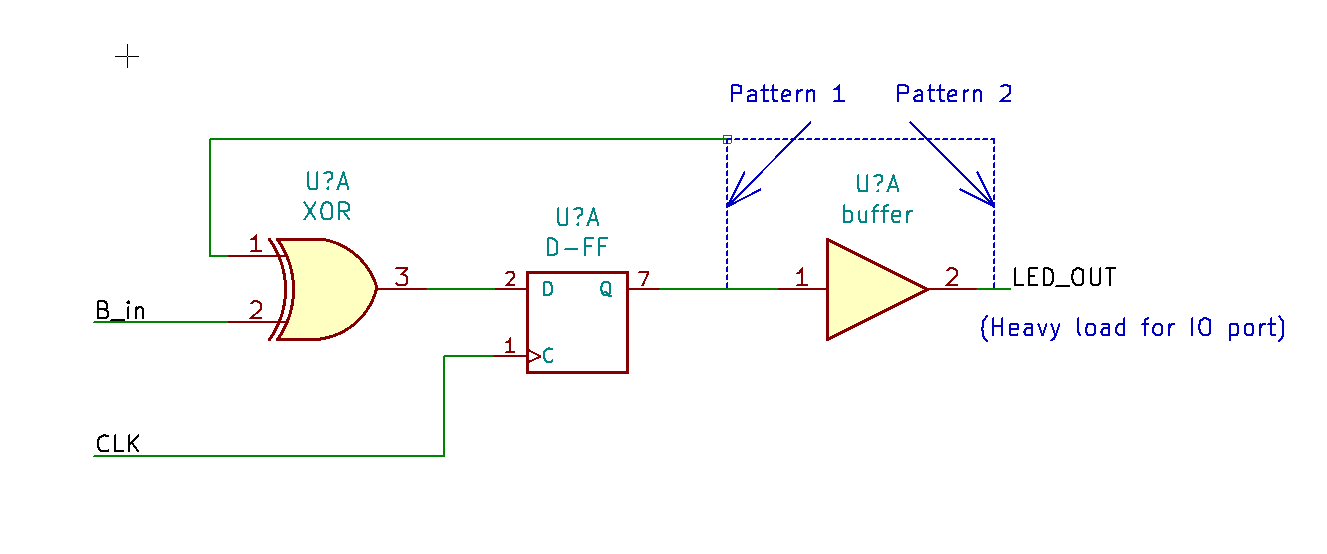
\includegraphics[angle=0,width=160mm]{week4/pics/io-port-whichistrue.png}
  \centering
  \caption{IOポートの構成によって結果が変わる例} %タイトルをつける
  \label{fig:io-config} %ラベルをつけ図の参照を可能にする
\end{figure}

ソースコードを付録のソースコード\ref{lst:no2-source}示す.

\subsection{課題3 LEDの点滅}
LED1個を1Hzで点滅させる.
クロック源のクロック周波数は50MHzなので 25'000'000回 カウントした段階でLEDをトグルさせることで実現できる.

ソースコードを付録のソースコード\ref{lst:ledblink-source}示す.

\subsection{課題4 7セグメントLEDの10進カウンタ}
押しボタンを押すたびに7セグメントLED1桁の値を 0 → 1 → 2 ... → 9 → 0 → ...と変化する回路を作成する.

押しボタンの入力には,チャタリングが含まれている可能性があるので,内部でチャタリング除去する必要がある.
また,押しボタンをトリガにイベントを起こすことは許されない.
クロック源は50[MHz]の発振器から供給し,それを分周した10[ms]程度のサンプリング周期でサンプリングを行い,チャタリングを除去する.

押下を判定するためには以前の状態を保持し,直前は押されず,今押されたことを確認する必要がある.
サンプリングした値をもとに,押下判定を行い,カウント動作を行う.

ソースコードを付録のソースコード\ref{lst:counter7seg10-source}示す.

\subsection{課題5 7セグメントLEDに1234を表示}
7セグメントLEDに「1234」を表示する回路を作成する.

7セグメントLEDは4桁表示でそれぞれの桁はアノードコモンで構成されている.
カソード側は同じタイプのセグメントが共有されていて,厳密に同時に複数の数字を表示することができない.

そのため高速に表示する桁を切り替えながら数字を一つずつ表示することであたかも同時に数字が表示されているかのように見えるようにする.
この方式をダイナミック点灯方式という.

約1msごとに桁を切り替え,4桁分表示するように設計する.
拡張性を考え,(課題6のため) モジュールとして汎用性がある形で設計する.

入力はクロックと表示する数値4桁分,出力は7セグメントLEDへの出力とする.

ソースコードを付録のソースコード\ref{lst:7seg1234-source}示す.

\subsection{課題6 4桁のカウンタの作成}
押しボタンを押すたびに7セグメントLEDの値が 0000 → 0001 → 0002 → ... → 9999 → 0000 → ... と変化する回路を作成する.
任意の位の桁上がりはその桁の現在の数値が9から0に変化するタイミングで発生し,それをもとに次の桁をインクリメントする.
残りの機能としては課題4と5を組み合わせて実装する.

ソースコードを付録のソースコード\ref{lst:10000-counter1}示す.

\subsubsection{課題6 除算器の制作}
実験が終わったあとに,解説を見た.10000進カウンタを作成し,
それをもとに割り算回路で商とあまりを求めて表示する方法が記述されていた.

それについても実装テストを行うべきだと判断し,実装することにする.
10000進カウンタを作るためには14ビット必要である.この数と10での除算を実装することで,
それぞれの桁を求めることができる.

10の割り算を実装する方法はいくつか提唱されている.例えば,単純に除算器を作成し,順に割っていく方法や,
逆数をかけて求める方法,
整数のシフトを順に繰り返していく方法\cite{int-div-const-2003}など,様々な方法がある.

割り算を行う除算器を作る方法や整数のシフトを順に繰り返していく方法は数サイクルを要するため,効率が悪い.
今回は短時間に処理が終わる,逆数を求める方法で計算をする.

解説と同じやり方ではなく,ここでは整数の乗算とシフトを用いた除算法を行う.
逆数を用いて乗算で計算する方法である.

まず10で割る必要があるので,10の逆数を求める.しかし単に求めるだけでは整数の丸め誤差が割り算の結果に悪影響があるので,ここでは固定小数点演算で計算する際のフォーマットの選定に注意が必要である.
固定小数点のフォーマットの選定は,必要な桁と割る数によって変える必要があるため,
この方法は定数の割り算ではよく使われるが定数以外の割り算では使われない.
固定小数点のフォーマットは小数点以下$N+log_2(M)$; Nはビット数,Mは割る数 で表現できる.
ここで切り捨て誤差を抑えるために,逆数で求めた値に1を足しておく.

この方法では,整数の丸め誤差が含まれるが,整数の範囲 (ビット数) を限定することで,誤差を小数点以下に追い込むことができる\cite{int-div-1937}.

今回は14ビットの数値を10で割った商と余りを求めているので,小数点以下17ビットの逆数を用いる.
つまりある数に13108をかけて,17ビットシフトすると10で割った商が求められる.

余りを求めるためには,この数を10でかけて差分を取ることで求められるが,多くのビットの計算になり,時間がかかる.
そのため,精度検証をしながら別の方法であまりを求める.
あまりとは,割ったときの小数部分をオフセットした値に比例する.
そのため割ったあまりをつかってある程度表現できる.
これが完璧ではないのは,すでに逆数に誤差が存在するためであるが,検証をした上で回路を記述することができる.
余りは割った数の小数点以下5ビットを10倍することで求めることができる\footnote{この方法は完璧ではなく,0から11263までしか誤差なく計算できないが,今回扱う数は$10^4-1$までなのでこのまま続けることにする}.

作成したモジュールを挙げる
\begin{itemize}
\item{10の除算器}
\item{プリスケーラ}
\item{7セグメントLED表示}
\item{カウンタ本体}
\end{itemize}

10の除算器は入力値を10で割った商と余りを出力する.

プリスケーラは50MHzのクロック信号を分周するのに使う.
クロック周波数を$\frac{1}{2}$から$\frac{1}{2^{24}}$までリニアに調節できるようになっている.\footnote{多くの場合クロックは分周ということから分母を整数で変更するが,今回は分子を変更し,クロック周波数を調節する.}

7セグメントLED表示モジュールへのクロック周波数を下げるとダイナミック点灯を目でも観測できる.

7セグメントLED表示モジュールは,入力値を表示する.
入力値は順に10で割られて余りは7セグメントLEDに出力する.
割った商は次の割る数にセットされ,次のクロック信号までに計算が完了する.
これを繰り返すことで7セグメントLEDに数値を表示することができる.

カウンタ本体はカウントをする.
カウントした数値を7セグメントLED表示モジュールへ出力する.

除算器を用いてた10000進カウンタのソースコードを付録のソースコード\ref{lst:10000-counter2}示す.

\subsection{課題7 $\Delta\Sigma$変調によるLEDの調光}
\subsubsection{デルタシグマ変調}
課題7は任意の回路を作成ということで,私はLEDの調光を行うことにした.

課題3ではディジタル的な点滅を行ったが,オンとオフの点滅である.
オンとオフの間でゆっくり変化させるためには調光を行う必要がある.
LEDの輝度をディジタル的に調光する方法として,よく使われる方式としてPWM方式\footnote{Pulse Width Modulationの略で,パルス幅変調のこと}がある.

PWM方式は安定した調光ができることが特徴である一方でEMC\footnote{Electro Magnetic Interferenceの略,電磁妨害のこと}対策としては特定の周波数に分布が偏るため有効ではない.
また,調光の分解能を上げるとPWMの周波数も下がるため,トレードオフの関係になる.

応答特性も悪い.周期が固定のため,周期ごとにしか値を変更できない.

今回採用した調光の方式は,デルタシグマ変調方式のディジタル変換である.
1ビットのデルタシグマ方式では,長期的に誤差が最小になるように出力が調整される.
1次遅延の場合,直前の出力の誤差成分を次の出力に伝搬させることで実現できる.

デルタシグマ変調方式の大きな特徴は,ダイナミックに変化する周波数で,
高い分解能と低い低周波数成分を実現できることが期待できる.
EMC対策として周波数を拡散することが有効であるが,
広い周波数に渡って周波数を拡散できるため有効な対策になる.

欠点としては,調光に必要な回路規模が大きくなることと,スイッチング回数の増大によるスイッチング損失の増大である.
PWMのように特定の周波数のみに対してのノイズ対策にはならないので,スイッチングの回路設計も煩雑になる.

\subsubsection{仕様}
デルタシグマ変調を実装するにあたり,必要なモジュールを挙げる.

\begin{itemize}
\item 分周器(プリスケーラ)
\item デルタシグマ変調器
\item テスト用モジュール
\end{itemize}

まず,分周器を設計する.
クロック信号が高速すぎるため,それを低速なクロックに分周するためのモジュールを用意する.
このモジュールでは,クロックを$\frac{(1+N)}{4096}$倍にするためのモジュールである.
Nは0~2047までの11ビットで,$\frac{1}{2}$から$\frac{1}{2048}$までリニアに分周できる.

デルタシグマ変調器では,分解能16ビットの変調器を生成する.
そのまま変調すると高速なシグナルができるが,LEDの出力にFPGAの出力をそのまま使うため,
少し周波数を落として使うために,分周器を用いて分周し,クロック周波数を調整する.
デルタシグマ変調方式では$17'h10000$を基準とし,現在の出力がそれ以上かそれ以下で論理レベルを決定する.
論理レベルを決定したあと,その誤差を現在の出力に加算する.

テスト用モジュールは,デルタシグマ変調が期待通りに動作しているかを検証するのに使う.
検証するのに4つのモードを用意する.
スライドスイッチでモードを自由に切り替えられるようにする.

1つ目はゆっくりLEDを点灯,消灯を繰り返すために0から65535まで出力をカウントアップし,そこから0までカウントダウンする.
カウントアップのトリガには別の分周器により分周したクロック信号を使う.

2つ目は出力を0(消灯)に固定,3つ目は,約40\%の出力,4つ目は100\%出力のテストを行う.

実験の手順としては,おおよその動作をシミュレーションする.
その後実際に実機で動かし,モードを変化させながらその様子の違いを観察する.


ソースコードを付録のソースコード\ref{lst:deltasigma}示す.


%% \clearpage
%==============================================
\section{実験結果}
\subsection{課題1 10進数カウンタの作成}
シミュレーション結果を図\ref{fig:counter10-testbench}に示す.
\begin{figure}[tbp]
  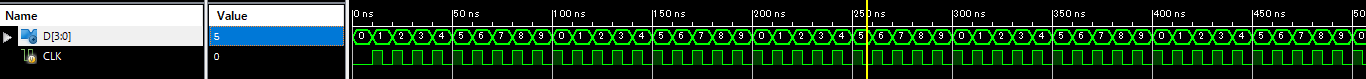
\includegraphics[angle=0,width=160mm]{week4/pics/counter10.png}
  \centering
  \caption{10進カウンタのテストベンチの結果} %タイトルをつける
  \label{fig:counter10-testbench} %ラベルをつけ図の参照を可能にする
\end{figure}

\subsection{課題2}
指で押しているときはLEDが半端な明るさになり,離すとLEDが点灯することもあれば消灯することもあった.
指を離した際にほぼ同じ確率でLEDがついたり消えたりした.

\subsection{課題3 LEDの点滅}
LEDが1秒周期で点滅した.

\subsection{課題4 7セグメントLEDの10進カウンタ}
7セグメントLEDがボタンを押すたびに 0 → 1 → ... → 9 → 0 → ... と変化した.

\subsection{課題5 7セグメントLEDに1234を表示}
7セグメントLEDに1234と出力できている.

\subsection{課題6 4桁のカウンタの作成}
0からカウントして2000程度まで手動で入力し,検証して,9999に初期値を設定して0に戻ることを確認した.
その他は検証していない.
\subsubsection{除算器を用いた方法での表示部のテストベンチ}
除算器のテストベンチの結果を図\ref{fig:div-testbench2}と図\ref{fig:div-testbench2}に示す.
Dが割る数で10で割った商(quotient)と余り(remainder)を出力している.
表示器のテストベンチの結果を図\ref{fig:display-testbench}に示す.
numは表示する数が入っていて,I1からI4に数字に対応する数が計算され,順に格納されている様子がわかる.
例えば21だとI4に1が,I3に2,それ以外は0が格納されている.

\begin{figure}[tbp]
  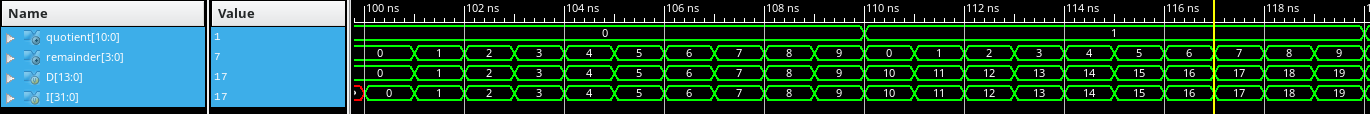
\includegraphics[angle=0,width=160mm]{week4/pics/div10-begin-testbench.png}
  \centering
  \caption{除算器のテストベンチ1} %タイトルをつける
  \label{fig:div-testbench1} %ラベルをつけ図の参照を可能にする
\end{figure}
\begin{figure}[tbp]
  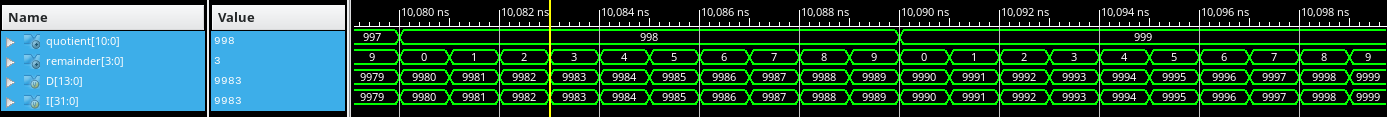
\includegraphics[angle=0,width=160mm]{week4/pics/div10-testbench.png}
  \centering
  \caption{除算器のテストベンチ2} %タイトルをつける
  \label{fig:div-testbench2} %ラベルをつけ図の参照を可能にする
\end{figure}
\begin{figure}[tbp]
  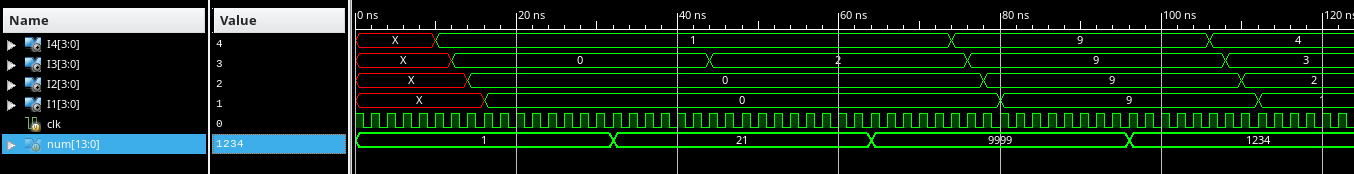
\includegraphics[angle=0,width=160mm]{week4/pics/10000decode.png}
  \centering
  \caption{表示機のテストベンチ} %タイトルをつける
  \label{fig:display-testbench} %ラベルをつけ図の参照を可能にする
\end{figure}


\subsection{課題7 $\Delta\Sigma$変調によるLEDの調光}
テストベンチを図\ref{fig:deltasigma-testbench1}と図\ref{fig:deltasigma-testbench2}に示す.

図\ref{fig:deltasigma-testbench1}では,最初のモードのゆっくり点滅するモードで,1周期の中から消灯部分付近を拡大した部分を出している.この変調方式の特徴である,パルスの密度が変化している様子がわかる.

図\ref{fig:deltasigma-testbench2}では,実際に波形が一定ではない部分を抜き出して示している.

実際に実機で動作させてみると,LEDをうまく調光できなかった.
画像等ではうまく表せないが,低周波発振を起こし,更に出力が両極端の時に不安定になった.

\begin{figure}[tbp]
  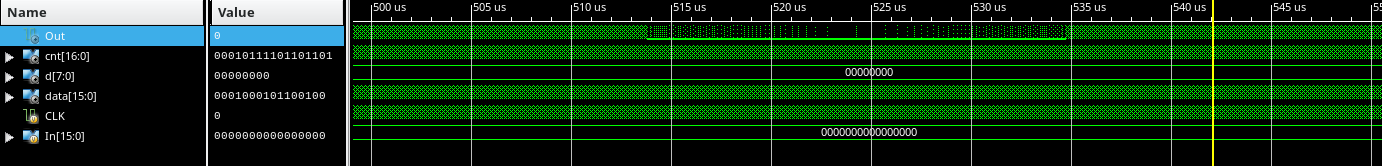
\includegraphics[angle=0,width=160mm]{week4/pics/deltasigma-sim.png}
  \centering
  \caption{$\Delta\Sigma$変調のテストベンチ1} %タイトルをつける
  \label{fig:deltasigma-testbench1} %ラベルをつけ図の参照を可能にする
\end{figure}
\begin{figure}[tbp]
  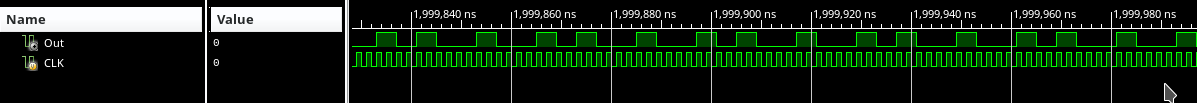
\includegraphics[angle=0,width=160mm]{week4/pics/deltasigma-waveform.png}
  \centering
  \caption{$\Delta\Sigma$変調のテストベンチ2} %タイトルをつける
  \label{fig:deltasigma-testbench2} %ラベルをつけ図の参照を可能にする
\end{figure}

\section{考察}
\subsection{課題1}
クロック信号の立ち上がりでカウントできていることが分かる.
0から9までカウントし,その後0に戻っている.

\subsection{課題2}
ボタンを押していても放した時の値はランダムに変化するようにみられたことから,図\ref{fig:io-config}中のPattern 2の方でコンフィグレーションが行われたのだと考えられる.
つまり,ポートの読み出しタイミングに関してLEDに出力する前にバッファが挟まっていて,
その前段階で,XORの入力部にフィードバックされていると考えられる.

\subsection{課題3 LEDの点滅}
LEDが1秒ごとに点滅した.
クロック源が正確であるため,安定した点滅のように見えた.

\subsection{課題4 7セグメントLEDの10進カウンタ}
10進カウンタの動作をした.
LEDが明く点灯したのは点灯しているLEDが1桁分だけのため,
4桁表示時よりも1桁に集中して電流が流れたためだと考えられる.

\subsection{課題5 7セグメントLEDに1234を表示}
7セグメントLEDの表示は,1234になった.
7セグメントLEDの桁を高速に切り替えることであたかも同時に表示されているかのように見えたのは,
目が高速な変化に追いついていないためだと考えられる.

\subsection{課題6 4桁のカウンタの作成}
2つの方法共にうまくカウントアップできた.
一つずつ考察していく.

\subsubsection{10進カウンタを工夫する方法}
この方法では,10進カウンタの動作以外に任意の数字を表示する機能は有さない.
そのため拡張性が低いと考えられる.

\subsubsection{除算器を使う方法}
除算器のテストベンチの結果,正しく10で割った商と余りを求められていることがわかる.

数値を各桁で分離するテストにも成功していることがわかる.
I1 から I4 に10進のそれぞれの数値が入っていることが読み取れる.

割り算回路は1つだけなので,順番に計算され,順に格納されているが,
この回路のダイナミック点灯方式では1桁ずつしか表示できないので,
割り算回路を1つ用意して順に割って余りを出せば十分である.

この方法では,回路は少々複雑になったが任意の4桁の数字を表示できた.
拡張が容易なため,拡張性が高いと考えられる.

割り算回路について考察していく. 
同様の計算を割り算回路で行うと,複数サイクル必要なので,1サイクルで終わる乗算器で逆数を求めたほうが効率が高い.
ただし,精度の考察が必要である点と,予め逆数を求める必要があるのが欠点である.
割る数に応じて回路構成を変更する必要がある.

\subsection{課題7 $\Delta\Sigma$変調によるLEDの調光}
テストベンチからは誤差がうまく分散している様子がわかる.
図\ref{fig:deltasigma-testbench2}でわかるように,この$\Delta\Sigma$変調方式では同じような出力範囲でも波形としてみるとHighとLowの幅が一定の出力にはならない.
常に累積誤差が最小になるように,出力が調節されるためである.

図\ref{fig:deltasigma-testbench1}でもその様子がよくわかる.
,最初のモードのゆっくり点滅するモードで,1周期の中から消灯部分付近を拡大した部分を出している.
この変調方式の特徴である,パルスの密度が変化している様子がわかる.

調光に関して,最初にテストベンチを書いて予想できたが,やはり実際の動作は不安定だった.
低周波発振も起きて,少しちらつきも見えた.
特に0\%や100\%付近の出力は,不安定になった.
これは$\Delta\Sigma$変調が交流信号向けだからだと思われる.
交流等価で見ると,PWMよりも特性が良くなることがあるものの,直流には精度が限定されたPWMが良いことが分かった.

%% \subsection{課題4 }xs

\clearpage
\section{感想}
FPGAによる同期回路の設計に関する基本的な知識を身につけられたと思う.
ハードウェアにとって実装が容易なタスク,そうでないタスクについて,振り分けを行い,ソフトウェアと共同して処理をすすめることがコンピュータの発展では欠かせないことがわかった.

\subsection{$\Delta\Sigma$変調について}
残りは,任意の回路を作成で,どんな回路を作るのか迷った.どうして$\Delta\Sigma$変調というマイナーな回路を作ることにしたのかについて説明しよう.

最初私はLEDをチカチカさせて終わりにしようかなって思ってた.しかしそれではつまらないと思い,もっと高度なことをしようと思った.

そこで,以前2年前だろうか,私は個人でPIC32MKシリーズを用いて
3ピンでNTSC\footnote{ビデオコンボジットの規格の一つ,昔のカラーテレビ放送の技術の一部に使われていた}シグナルを
生成する試みを行ったことがあった.
そこでは,参考にした文献の中に1ピンでNTSCシグナルを生成する試みがあった.
FPGAは200MHz付近の高速なシグナル生成でビット精度を稼いでいたがマイコンでは50MHz付近までしか使えない.
代わりに3ピンだったらシグナル生成できるのではと考えたのがきっかけだった.
3ビットのDACの出力ではもちろんカラーコンボジット入力のカラーバースト信号ですらもうまく生成できない.
制約をパスするためには3ビットの入力をうまく変調して誤差を分散する必要があった.
ここでは1次の$\Delta\Sigma$フィルタを用いて誤差分散をかけた.
1波長を16回出力に設定した.1ドットを$\frac{1}{2}$波長分,つまり8回出力にした.
この方法では4:3スクリーンでは正方ドットにはならないが,ワイドスクリーンではほぼ正方ドットになる.

NTSCシグナルの生成はうまくいった.
カラービデオ出力に成功し,3ビットのDACの難点であったカラー精度も時間を高速にしたことにより,幾分も改善することができた.
この成功の影には,$\Delta\Sigma$方式のDAコンバータとNTSCシグナルの相性が良かったことが言えるだろう.
NTSCシグナルは$fsc=3.579545$[MHz]の基本周波数をもち,鋭い遮断特性を持つフィルタによりフィルタリングされる.
このおかげでそのこの基本周波数の16倍のサンプリング周波数で出力したシグナルは安定してテレビに出力できた.

ただ,今回の実験でもうまく行くかと思った.直流ではそう簡単には行かないようだ.
そのことがわかって,PWM技術の長所を改めて実感することができた.

\subsection{最後に}
FPGAは前から興味を持ちながら,高額なハードウェア,それからソフトウェアライセンスにより,意欲が削がれていた.
そういう自分を情けなく思うこともあり,高専時代の卒業研究では,FPGAを用いた研究をしようとしてたのだ.
しかし卒業研究をすすめるうちに自分のやるべきこと,やらなくてはならないことが明確になり,FPGAを触るのをやめてしまった.

ハードウェアは可能性が大きい.そのため今後も継続してハードウェアとソフトウェアの共存について研究していきたいと思う.

\clearpage
\section{付録}

\lstinputlisting[caption=課題1 ソースコード,label=lst:10counter-source]{week4/source/counter.v}
\lstinputlisting[caption=課題1 テストベンチ,label=lst:10counter-testbench]{week4/source/countertestbench.v}
\lstinputlisting[caption=課題2 ソースコード,label=lst:no2-source]{week4/source/no2.v}
\lstinputlisting[caption=LEDの点滅のソースコード,label=lst:ledblink-source]{week4/source/ledblink.v}
\lstinputlisting[caption=7セグメントLED10進カウンタソースコード,label=lst:counter7seg10-source]{week4/source/counter7seg10.v}
\lstinputlisting[caption=7セグメントLEDに1234表示ソースコード,label=lst:7seg1234-source]{week4/source/led7seg.v}
\lstinputlisting[caption=4桁のカウンタ,10進カウンタを組み合わせる方法のソースコード,label=lst:10000-counter1]{week4/source/ledcounter10000.v}
\lstinputlisting[caption=4桁のカウンタ,10000進カウンタと除算器を組み合わせる方法のソースコード,label=lst:10000-counter2]{week4/source/counterdivver.v}
\lstinputlisting[caption=$\Delta\Sigma$方式の調光ソースコード,label=lst:deltasigma]{week4/source/deltasigma.v}


\addcontentsline{toc}{chapter}{参考文献}
\begin{thebibliography}{9}
\bibitem{int-div-const-2003} Henry S. Warren,INTEGER DIVISION BY CONSTANT,Chapter 10,Hacker's Delight (2nd Edition) ,2003年
\bibitem{int-div-1937} Hasselstrom, Karl,Fast Division of Large Integers: A Comparison of Algorithms,Master's in Computer Science thesis,Royal Institute of Technology,1994年
\end{thebibliography}


\end{document}
